\subsection*{Groep IO}
\begin{itemize}
\item Tutorials gevolgd en onszelf geoefend in WebGL. Het resultaat is te zien in figuur \ref{fig:WebGL}.
\item PHP basic authentication afgemaakt, er wordt nu gecheckt of de username/password combinatie bestaat. Het inlogscherm dat interactie heeft met de PHP is te zien in figuur \ref{fig:login}.
\item Begin gemaakt aan HTML pagina 'reserveren app: buttons zijn toegevoegd
\end{itemize}

\subsubsection*{Volgende week}
\begin{itemize}
\item Begin maken aan media website en gebruikmaken van de opgedane kennis van WebGL.
\item Indien HTTPS beschikbaar is, het afmaken van het authenticatiesysteem met veilige en versleutelde verbinding
\item Verder gaan met indelen van end user dashboard
\item Gegevens van de server laten zien in het end user dashboard
\end{itemize}


\begin{figure}[htbp]
\centering
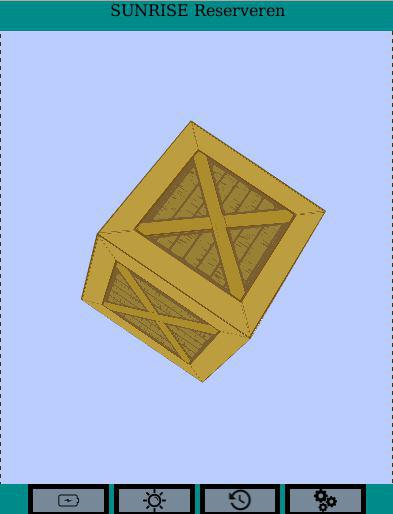
\includegraphics[width=5cm]{images/WebGL.jpg}
\caption{WebGL demo}\label{fig:WebGL}
\end{figure}

\begin{figure}[htbp]
\centering
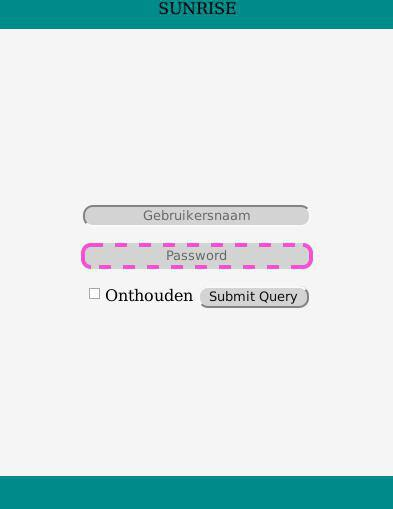
\includegraphics[width=5cm]{images/login.jpg}
\caption{Login pagina}\label{fig:login}
\end{figure}
